\section*{Systemtheorie der Sinnesorgane}
\setcounter{subsection}{4} 
\subsection{Übung}
\subsubsection{Zwei-Dimensionale Fourier Transformation}
In dieser Aufgabe wurde eine zweidimensionale Fouriertransformation  (Fig. \ref{fig:1b}) eines Bildes (Fig. \ref{fig:1a}) mit den Ortsfrequenzen $f_x = \frac{0.1}{\mathrm{Pixel}}$ in horizontale und $f_y = \frac{0.2}{\mathrm{Pixel}}$ in vertikale Richtung berechnet. Dazu wurde ein 30x30 Pixel großes Gebiet nach der Formel $Z(x,y)\ =\ \cos(f_x \cdot x\ +\ f_y\cdot y)$ erstellt und mit einem Gleichanteil von 1 in ausschließlich positive Werte konvertiert.

\begin{figure}[h]
    \captionsetup{width=0.8\columnwidth}
    \centering
    
\includegraphics[width=.4\columnwidth]{ue5/1a.eps}
    \caption{Computergeneriertes Bild (30x30 px) mit den Ortsfrequenzen $f_x = \frac{0.1}{\mathrm{Pixel}}$ in horizontale und $f_y = \frac{0.2}{\mathrm{Pixel}}$ in vertikale Richtung.}
    \label{fig:1a}
\end{figure}

\subsubsection{Problem 1 b}
Von dem Bild aus Fig. \ref{fig:1a} wurde nun eine 2D-Diskrete Fouriertransformation (\textit{2D-DFT}) berechnet und logarithmisch skaliert. Wie diese zeigt, sind im symmetrischen Frequenzraum drei Maxima sichtbar. Das Maximum in der Mitte des Bildes entspricht hierbei dem Gleichanteil, die beiden äußeren Maxima links oben und rechts unten stellen im Absolutwert die initialen Ortsfrequenzen in beide Dimensionen dar.
\begin{figure}[h]
    \captionsetup{width=0.8\columnwidth}
    \centering
    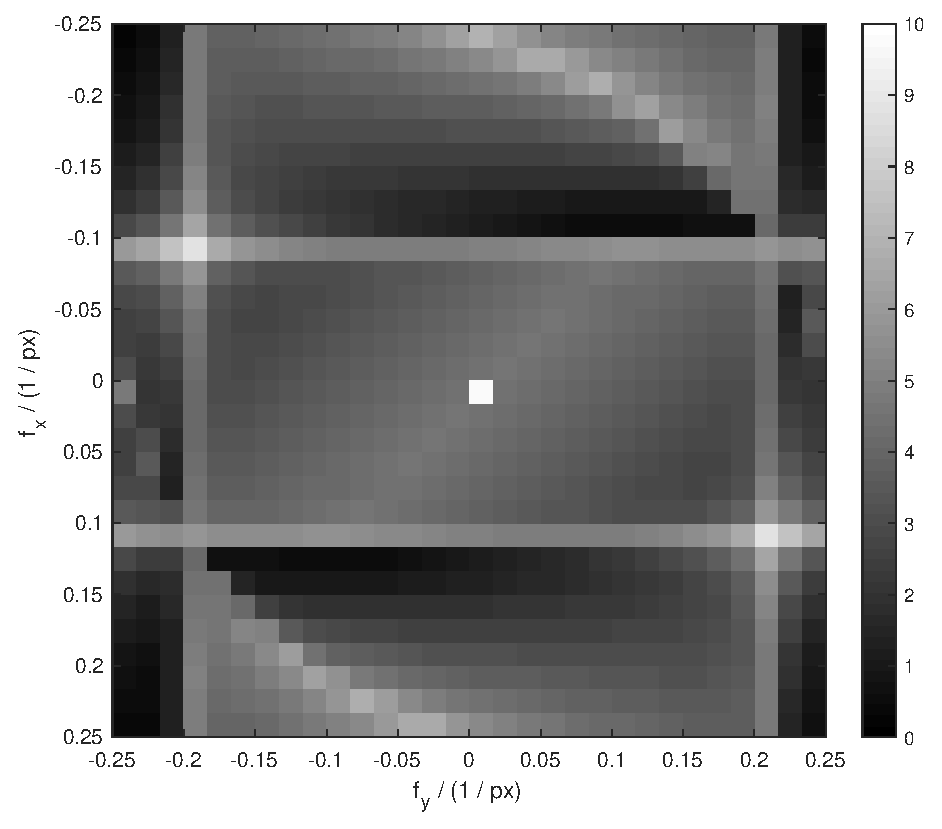
\includegraphics[width=.4\columnwidth]{ue5/1b.eps}
    \caption{2D-DFT des generierten Bildes aus Abbildung \ref{fig:1a}.}
    \label{fig:1b}
\end{figure}

\subsubsection{Problem 1 c}

Der kürzeste Abstand $d_{min}$ zwischen zwei parallelen Geraden kann durch eine Linie, die senkrecht auf beide Geraden steht, ermittelt werden. Hierbei wird ein rechtwinkliges Dreieck angenommen, das aus der Ankathete $a = \frac{1}{f_x}$, der Gegenkathete $g = \frac{1}{f_y}$, der Hypotenuse $h = \sqrt{a^2+g^2}$, sowie der Höhe $d_{min}$ besteht. Die Fläche des Dreiecks beträgt somit: $A = \frac{1}{2} a g = \frac{1}{2} d_{min} h = \frac{1}{2} d_{min} \sqrt{a^2 + g^2}$.
\vspace{2pt}
Geometrische Überlegungen ergeben:
$$d_{min} = \frac{a g}{\sqrt{a^2 + g^2}} = \frac{\frac{1}{f_x} \cdot \frac{1}{f_y}}{\sqrt{\frac{1}{f_x^2} + \frac{1}{f_y^2}}} = \sqrt{\frac{1}{\frac{f_x^2 \cdot f_y^2}{f_x^2} + \frac{f_x^2 \cdot f_y^2}{f_y^2}}} = \sqrt{\frac{1}{f_y^2+fx^2}}$$

\begin{figure}[h]
    \captionsetup{width=0.8\columnwidth}
    \centering
    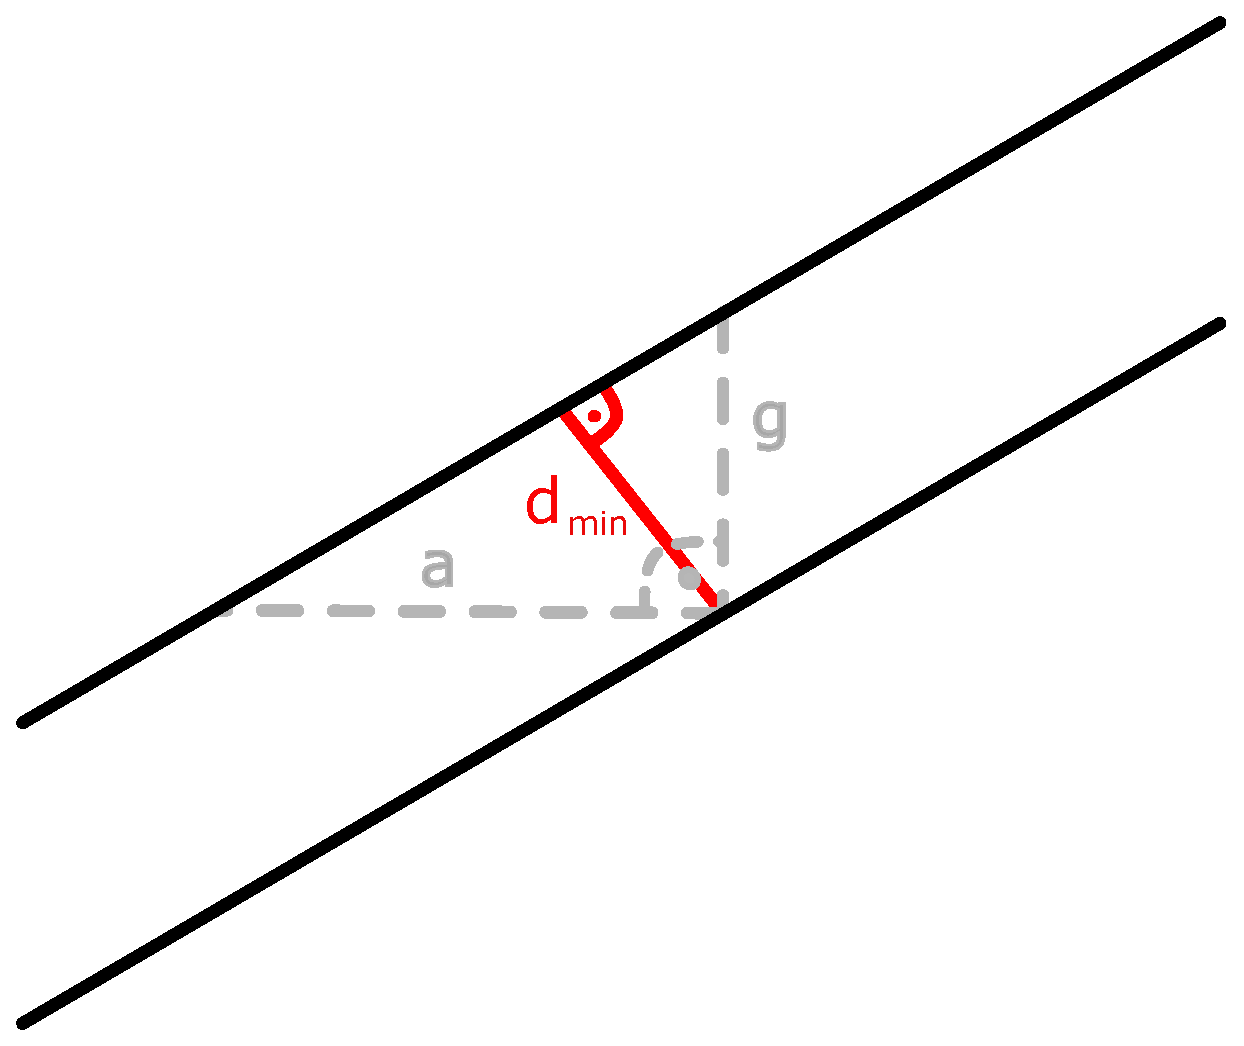
\includegraphics[width=.4\columnwidth]{ue5/Dmin.eps}
    \caption{Schema der obigen Herleitung. Die grauen Striche stellen die bekannten Parameter dar: a bedeutet im realen Bild eine Distanz von $\frac{1}{f_x}$, während b zu einer Distanz von $\frac{1}{f_y}$ korrespondiert. $d_{min}$ kann dann über die obige Formel berechnet werden.}
    \label{fig:Dmin}
\end{figure}

Daher ist $d_{min} = 1 \div \sqrt{f_y^2+fx^2} = 4.4721 \text{px}$ Dies führt zu einer Frequenz $f_{min} = \frac{1}{d_{min}} = \sqrt{f_x^2+f_y^2} = 0.2236 \frac{1}{\text{px}}$.

\subsubsection{Problem 2 a}

Siehe separate Abgabe.


\subsubsection{Problem 2 b}
% Mit welcher frequenz wird die helligkeit eines pixels moduliert

Die Intensität alias Helligkeit des Bildes ist gemäß der nachfolgenden Formel definiert:
$$I(x,y,t) = \cos( f_t \cdot t + f_x \cdot x)$$
Für einen einzelnen Pixel des Bildes sind die Ortkoordinaten konstant. Somit ergibt sich für einen Punkt des Bildes die vereinfachte Formel:
$$I_{x,y}(t) := I(x,y,t) \big|_{x,y = \text{const}} = \cos(f_t \cdot t + f_x \cdot x) \big|_{x=\text{const}} = \cos(f_t \cdot t + x_0)$$
Eine Periode dieses Cosinus-Signals hat die Länge $2 \pi$. Somit dauert ein Durchlauf des vertikalen Balkens durch das Bild $2\pi \div f_t$ Sekunden. Die Frequenz der Intensität/Helligkeit eines Pixels kann durch obige Formel als $f_t$ identifiziert werden.

\subsubsection{Problem 3 a}
Das eindimensionale, ideale Tiefpassfilter ist im Frequenzbereich ein Rechteck mit der Funktion \begin{equation*}
H(f)\ =\ \operatorname{rect}(t) = \sqcap(t) = \begin{cases}
0           & \text{wenn } \big|\frac{f}{2B}\big| > \frac{1}{2} \\[3pt]
\frac{1}{2} & \mbox{wenn } \big|\frac{f}{2B}\big| = \frac{1}{2} \\[3pt]
1           & \text{wenn } \big|\frac{f}{2B}\big| < \frac{1}{2}
\end{cases}
\end{equation*} wobei $B$ die Grenzfrequenz des Filters beinhaltet.

Bei einer Transformation in den Zeitbereich kann die Impulsantwort dann als Sinc-Filter angesehen werden: \begin{equation*}
    h(t) = \mathcal{F}^{-1} \{ H \}(t) = 2B\cdot \frac{\sin(2\pi Bt)}{2\pi Bt} = 2B\cdot \mathrm{si}(2\pi Bt)
\end{equation*}


\subsubsection{Problem 3 b}
In Abbildung 4A ist das \textit{Bricks} Bild dargestellt. Auf diesem Bild ist eine geziegelte Mauer mir markanten horizontalen, sowie vertikalen Linien dargestellt. Folglich kann ausgesagt werden, dass das Bild einige höherfrequente direkt horizontale und vertikale Muster enthält. In Abbildung 4B ist das $2D$-FFT transformierte, logarithmische Amplitudenspektrum des Bildes dargestellt. Markant ist dort die vertikale Linie nahe der horizontalen Mitte des Bildes. Diese spiegelt die markanten horizontalen Linien des Bildes wider.

Ebenso erkennbar, aber nicht so markant, ist eine horizontale Linie in Abbildung 4B nahe der vertikalen Mitte des Bildes zu erkennen. Diese spiegelt die vertikalen Linien des Bildes wider. Da diese im Gegensatz zu den horizontalen Linien im Bild kürzer, versetzter und unterbrochener sind, ist diese Attitüde nicht derart markant im Spektrum zu erkennen. Durch das reguläre bzw. repetitive Muster im Ausgangsbild, ergibt sich außerdem ein Matrix-ähnliches Muster im Frequenzbereich. 

\begin{figure}[!h]
\centering
\begin{subfigure}[b]{0.45\textwidth}
    \centering
    
\includegraphics[width=\textwidth]{ue5/bricks_im.eps}
    \caption{Bricks Bild.}
    \label{fig:bricks_im}
\end{subfigure}
\begin{subfigure}[b]{0.45\textwidth}
    \centering
    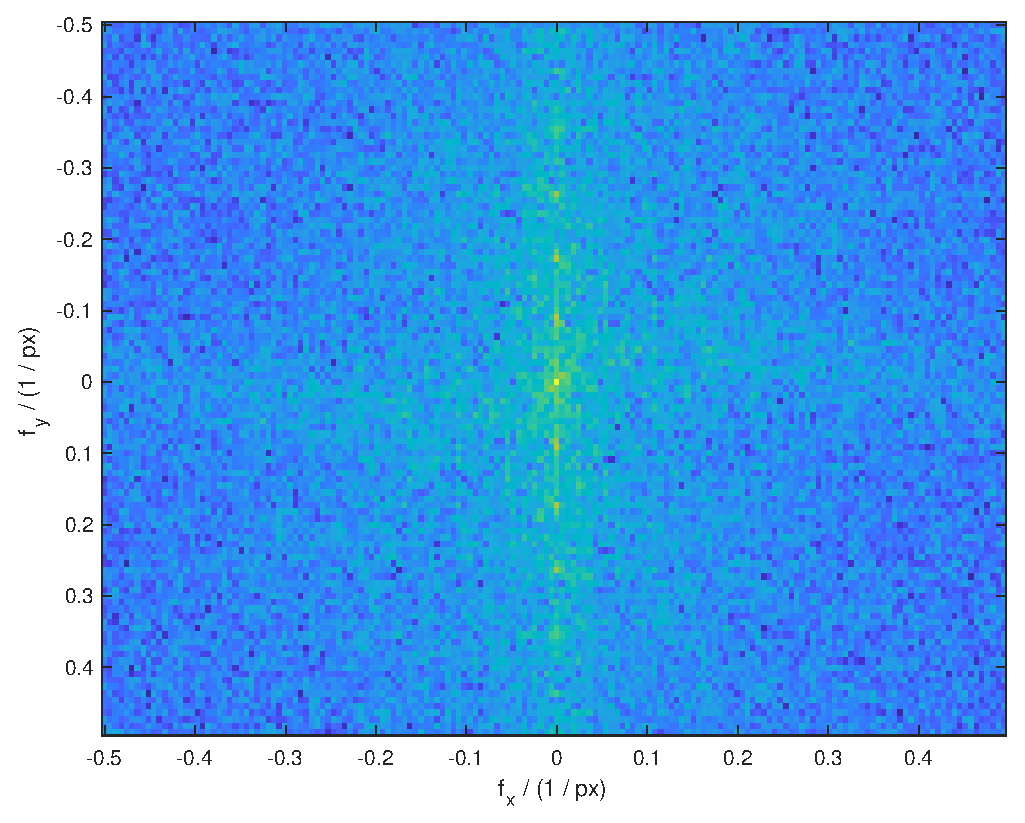
\includegraphics[width=.85\textwidth]{ue5/bricks_spec.eps}
    \caption{Bricks Spektrum.}
    \label{fig:bricks_spec}
\end{subfigure}
\label{fig:bricks}
\caption{Ausgangsbild und logarithmisches Amplitudenspektrum des Bricks Bildes.}
\end{figure}

In Abbildung 5A ist das \textit{Alhambra} Bild dargestellt. Dieses besteht aus verschiedenen geometrischen Formen, die jedoch regulär angeordnet sind. Die Anordnung ist markant entlang der Bilddiagonalen zu finden. Wie bereits in Aufgabe 1 gezeigt bestehen diagonale Linien auf einer horizontalen und vertikalen Komponente. Diese spiegeln sich im Amplitudenspektrum als horizonale und vertikale Linien wieder, die jedoch besonders ausgeprägte Punkte an deren Schnitten haben. Folglich beschreiben die zahlreichen Punkte im Amplitudenspektrum des Alhambra Bildes die diagonalen Züge des Bildes.  


regelmäßige Punktwolke um Null mit vertikalen Linien
Siehe erste aufgabe: diagonale Linie
\begin{figure}[!h]
\centering
\begin{subfigure}[b]{0.45\textwidth}
    \centering
    
\includegraphics[width=\textwidth]{ue5/alhambra_im.eps}
    \caption{Alhambra Bild.}
    \label{fig:alhambra_im}
\end{subfigure}
\begin{subfigure}[b]{0.45\textwidth}
    \centering
    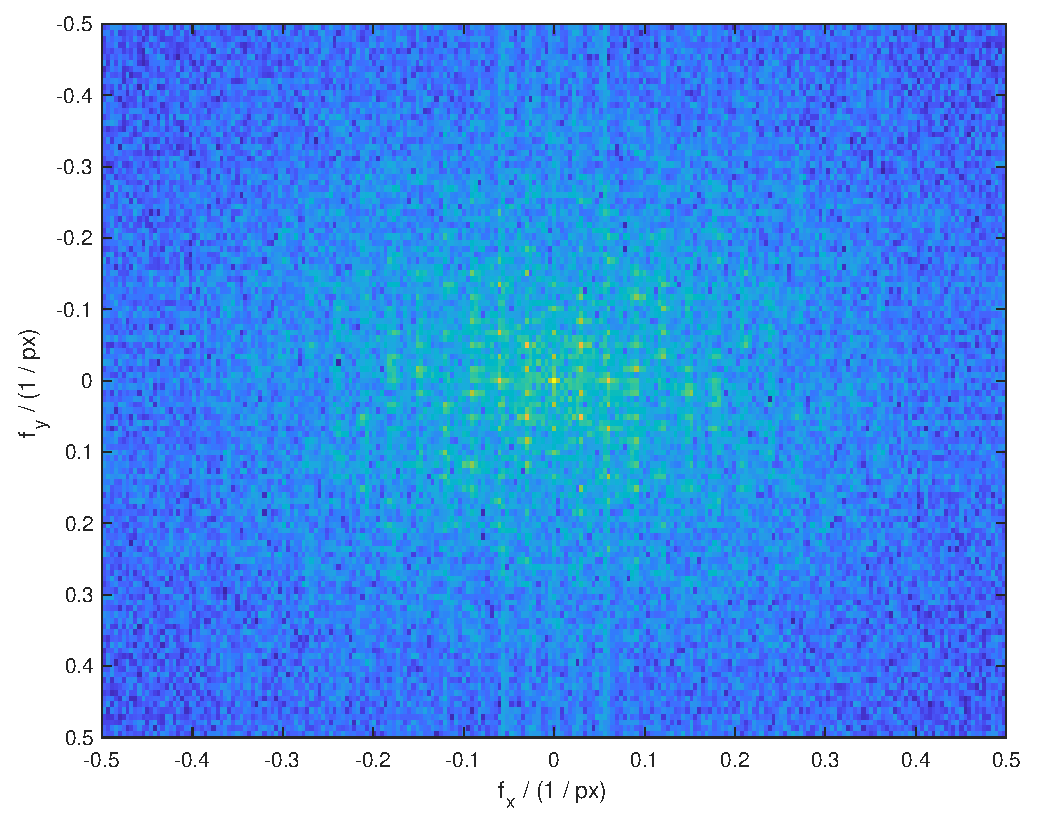
\includegraphics[width=.85\textwidth]{ue5/alhambra_spec.eps}
    \caption{Alhambra Spektrum.}
    \label{fig:alhambra_spec}
\end{subfigure}
\label{fig:alhambra}
\caption{Ausgangsbild und logarithmisches Amplitudenspektrum des Alhambra Bildes.}
\end{figure}

\subsubsection{Problem 3 c}
Hier wurden die Bilder im Frequenzbereich bis zu einer Grenzfrequenz von $B = \frac{0.13}{\mathrm{Pixel}}$ mit einem Tiefpass gefiltert. Dadurch ergibt sich eine Unschärfe, die durch den Verlust der - in den hohen Frequenzen enthaltenen - Detailinformation bedingt ist. Durch die Regularität des \textit{Alhambra} Bildes sowohl im Zeit-, als auch im Frequenzbereich, werden dessen Features durch das Filter im Vergleich zum \textit{Bricks} nicht so stark beeinflusst.
\begin{figure}[!h]
    \centering
    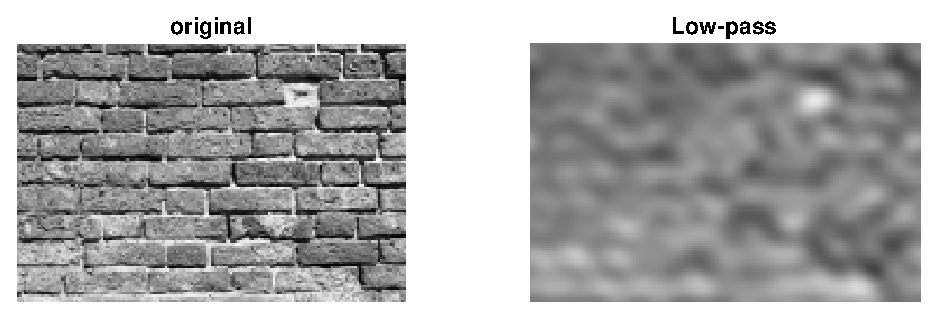
\includegraphics[width=\textwidth]{ue5/bricks_lp.eps}
    \caption{Filtered Bricks Image.}
    \label{fig:bricks_lp}
\end{figure}

\begin{figure}[h]
    \captionsetup{width=0.8\columnwidth}
    \centering
    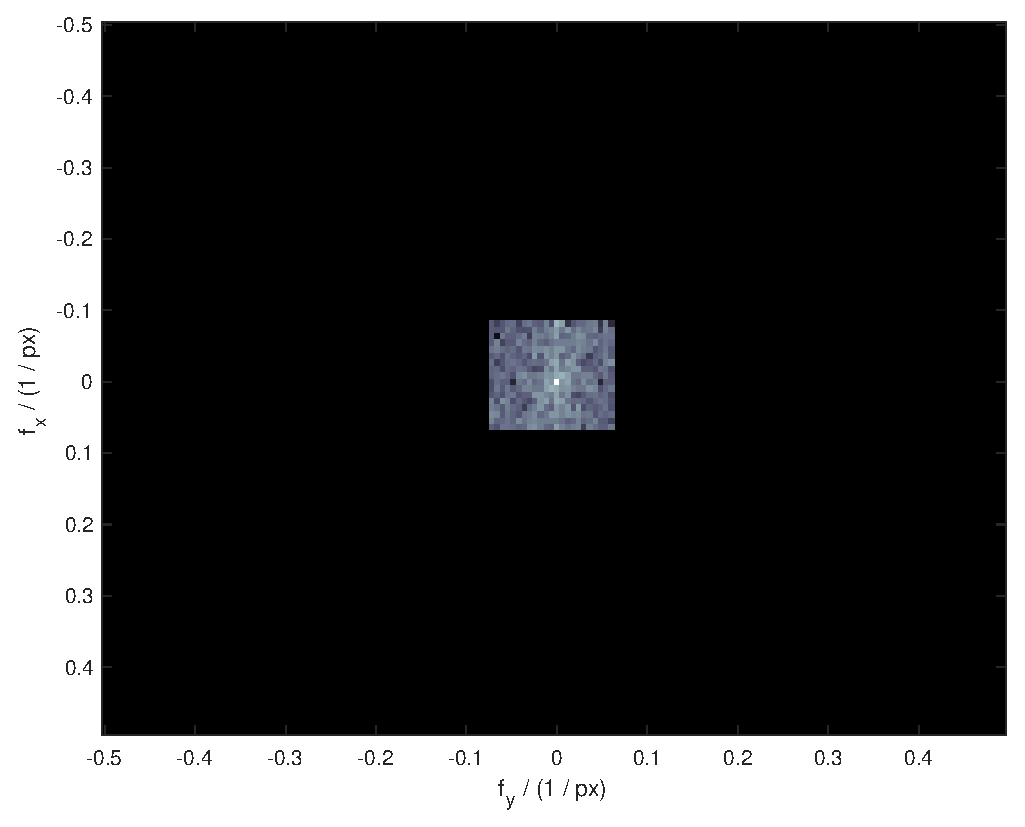
\includegraphics[width=.4\columnwidth]{ue5/bricks_spec_fil.eps}
    \caption{Amplitudenspektrum des gefilterten Bricks Bildes.}
    \label{fig:bricks_lp_fil}
\end{figure}

\begin{figure}[!h]
\centering
    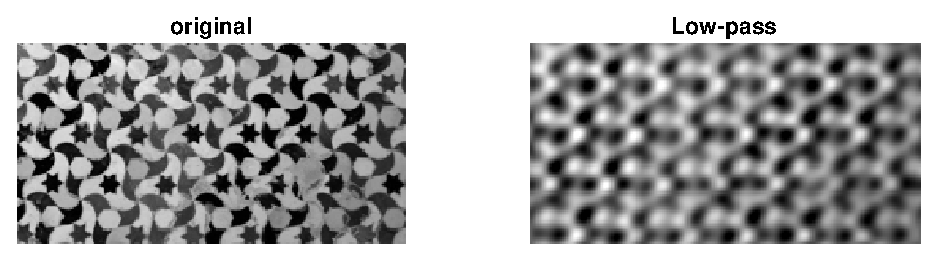
\includegraphics[width=\textwidth]{ue5/alhambra_lp.eps}
    \caption{Filtered Alhambra Image.}
    \label{fig:alhambra_lp}
\end{figure}

\begin{figure}[h]
    \captionsetup{width=0.8\columnwidth}
    \centering
    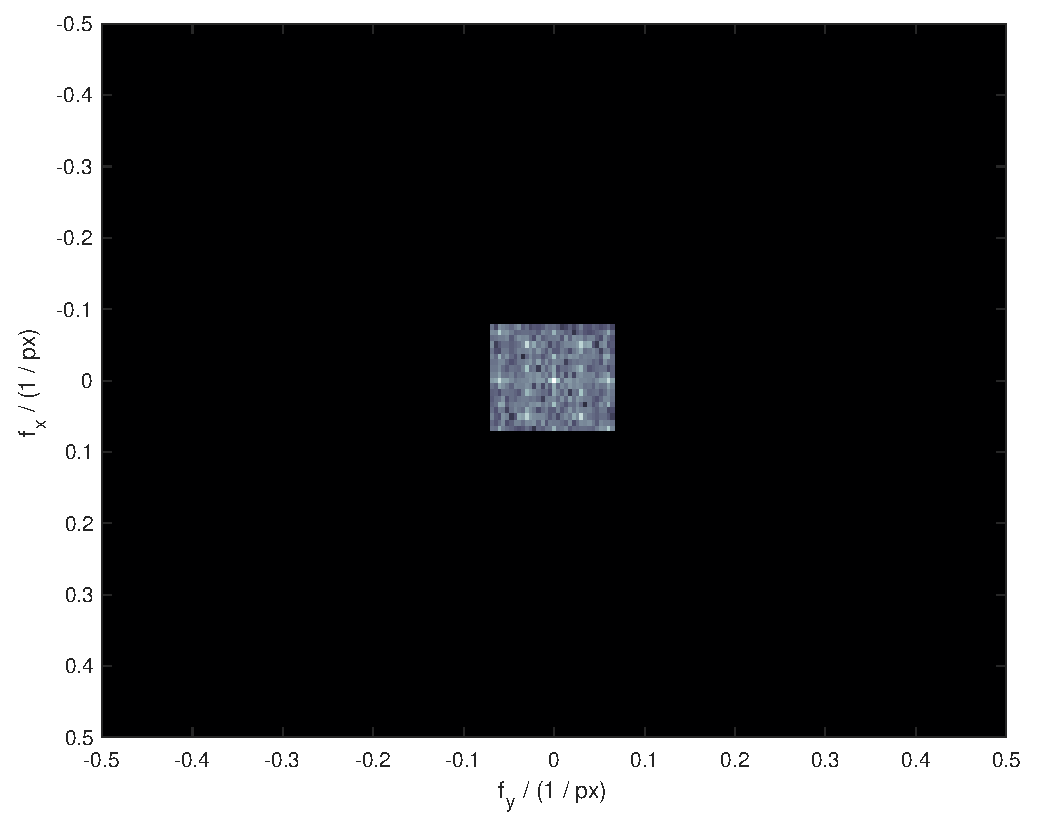
\includegraphics[width=.4\columnwidth]{ue5/alhambra_spec_fil.eps}
    \caption{Amplitudenspektrum des gefilterten Alhambra Bildes.}
    \label{fig:alhambra_lp_fil}
\end{figure}